\chapter{Build Management/ System Building}

Hat man nun den Quellcode der einzelnen Software Komponenten in dem Software- Projekt erstellt, dann möchte man diesen ausführbar machen. Hierum kümmert sich der Build Prozess. Dieser Prozess ist zuständig für das Kompilieren und Linking der einzelnen Software Komponenten in ein ausführbares System. Da die Abhängigkeiten von den Quellcodes, Bildern und weiteren Artefakten bei großen Projekten sehr komplex und unübersichtlich sind, empfiehlt es sich, diese Abhängigkeiten nicht alle manuell zu kompilieren. Hinzu kann natürlich noch kommen, dass für unterschiedliche Systeme unterschiedliche Kombinationsmöglichkeiten von Einzelkomponenten für den Build Prozess benötigt werden. Man erkennt also, dass das einfache Kompilieren von Quellcode für ein Software Projekt nicht ausreicht, sondern man weitreichende Überlegungen dazu anstellen muss.
\\
Für diesen Build Schritt in der Softwareentwicklung gibt es inzwischen Unterstützung von automatischen Tools. 
Diese Tools enthalten meistens eine Abhängigkeitsspezifikationssprache und einen Interpreter für  diese Sprache. Ebenso ist meist noch die Möglichkeit zur verteilten Kompilation, die Auswahl von Tools und Support für die Instanziierung des Softwareprojektes gegeben. 
\\
Das bekannteste Tool für UNIX ist make für die C/C++ Entwicklung. Make ist dafür zuständig die Abhängigkeiten zwischen Sourcecode und Objektcode zu beobachten und re-kompiliert automatisch die Sourcen welche nach dem Erstellungsdatum des zugehörigen Objektcodes verändert wurden. Die Abhängigkeiten werden in Makefiles abgebildet, wie auch im folgenden Code ersichtlich wird:

\lstinputlisting[style=makefile,label=makefile,caption=Makefile für Speicherverwaltung aus Systemnahe Software 1-WS 2013/14]{code/Makefile}

In Listing \ref{makefile} werden zuerst die Quellen, die Objekte (die Abhängigkeiten) und die Zielquelle definiert, ebenso der benötigte Kompiler mit Option.
Anschließend werden die einzelnen Befehle beschrieben, also was passiert bei dem Aufruf von \textit{make clean, make realclean} und \textit{make depend}. In den Zeilen 15-17 findet man dann die einzelnen Abhängigkeiten, die mit make depend gefunden wurden.
\\
Weitere bekannte Tools sind Apache Ant, das wohl häufigste verwendete Tool für Java, das analog zu make in einer Datei build.xml die Abhängigkeiten beschreibt, Maven (ebenfalls Java), Jam, MS Build (.NET) und scons.
Doch auch an solche automatischen Tools gibt es eine Anforderungsliste. 
\cite{bib:se}
\begin{itemize}
\item Enthalten die Build Anweisungen alle benötigten Komponenten ?
\item Ist für jede Einzelkomponenten die richtige Version spezifiert?
\item Sind alle benötigten Dateien verfügbar ?
\item Sind die Referenzen innerhalb der Komponenten richtig, also ruft die eine Komponente eine andere mit den richtigen Parametern und Namen auf?
\item Wird die Software auch für das richtige Betriebssystem erstellt?
\item Mit welcher Kompilerversion und weiteren benötigten Software-Tools wird dieser Build-Prozess durchgeführt? 	
\end{itemize}

\section{Continous Build}
Schnell stellt sich jedoch die Frage wie oft denn ein solcher Build Prozess durchgeführt werden soll? Soll er nach jeder Änderung, jeder fertigen Teilkomponente durchgeführt werden, um die Funktionen zu testen, oder soll erst am Ende vom Projekt ein kompletter Durchlauf des Build-Prozesses durchlaufen?
\\
Hierfür gibt es keine richtige und falsche Antwort. Die sollte je nach Komplexität des Softwareprojekts individuell entschieden werden. Denn ein solcher Build Prozess kann je nach Komplexität der zu erstellenden Software sehr rechenintensiv und lange sein. 
\\
Zum einen wird ein Build aufwendiger, je seltener dieser durchgeführt wird, da die Fehlerwahrscheinlichkeit steigt und die Einzelkomponenten der Software auseinander laufen können.
\\
Anderseits wiederum ist das ein Nachteil wenn man den Build zu oft durchführt, da bei großen Software Projekten viele Ressourcen benutzt werden, die der Build zu berücksichtigen hat und somit immer rechenintensiver wird.
\\
Die optimale Strategie muss für jedes Softwareprojekt individuell gefunden werden.
Wenn man nach jeder Änderung ein Build durchführen möchte, 
dann bezeichnet man dies als Continuous Integration.
Durch Verwendung von Tools kann hierbei eine Überwachung der Ressourcen und der Aufruf des Build-Tools automatisiert werden. Ebenso kann die Automatisierung des Test nach dem erfolgten Build erfolgen. \cite{build-seminar}, \cite{software-analysis}
\\
Im der folgenden Abbildung \ref{fig:ci} sieht man die Abhängigkeiten, die in einem Software-Projekt vorliegen, darunter auch den Build Prozess.

\begin{figure}[H]
	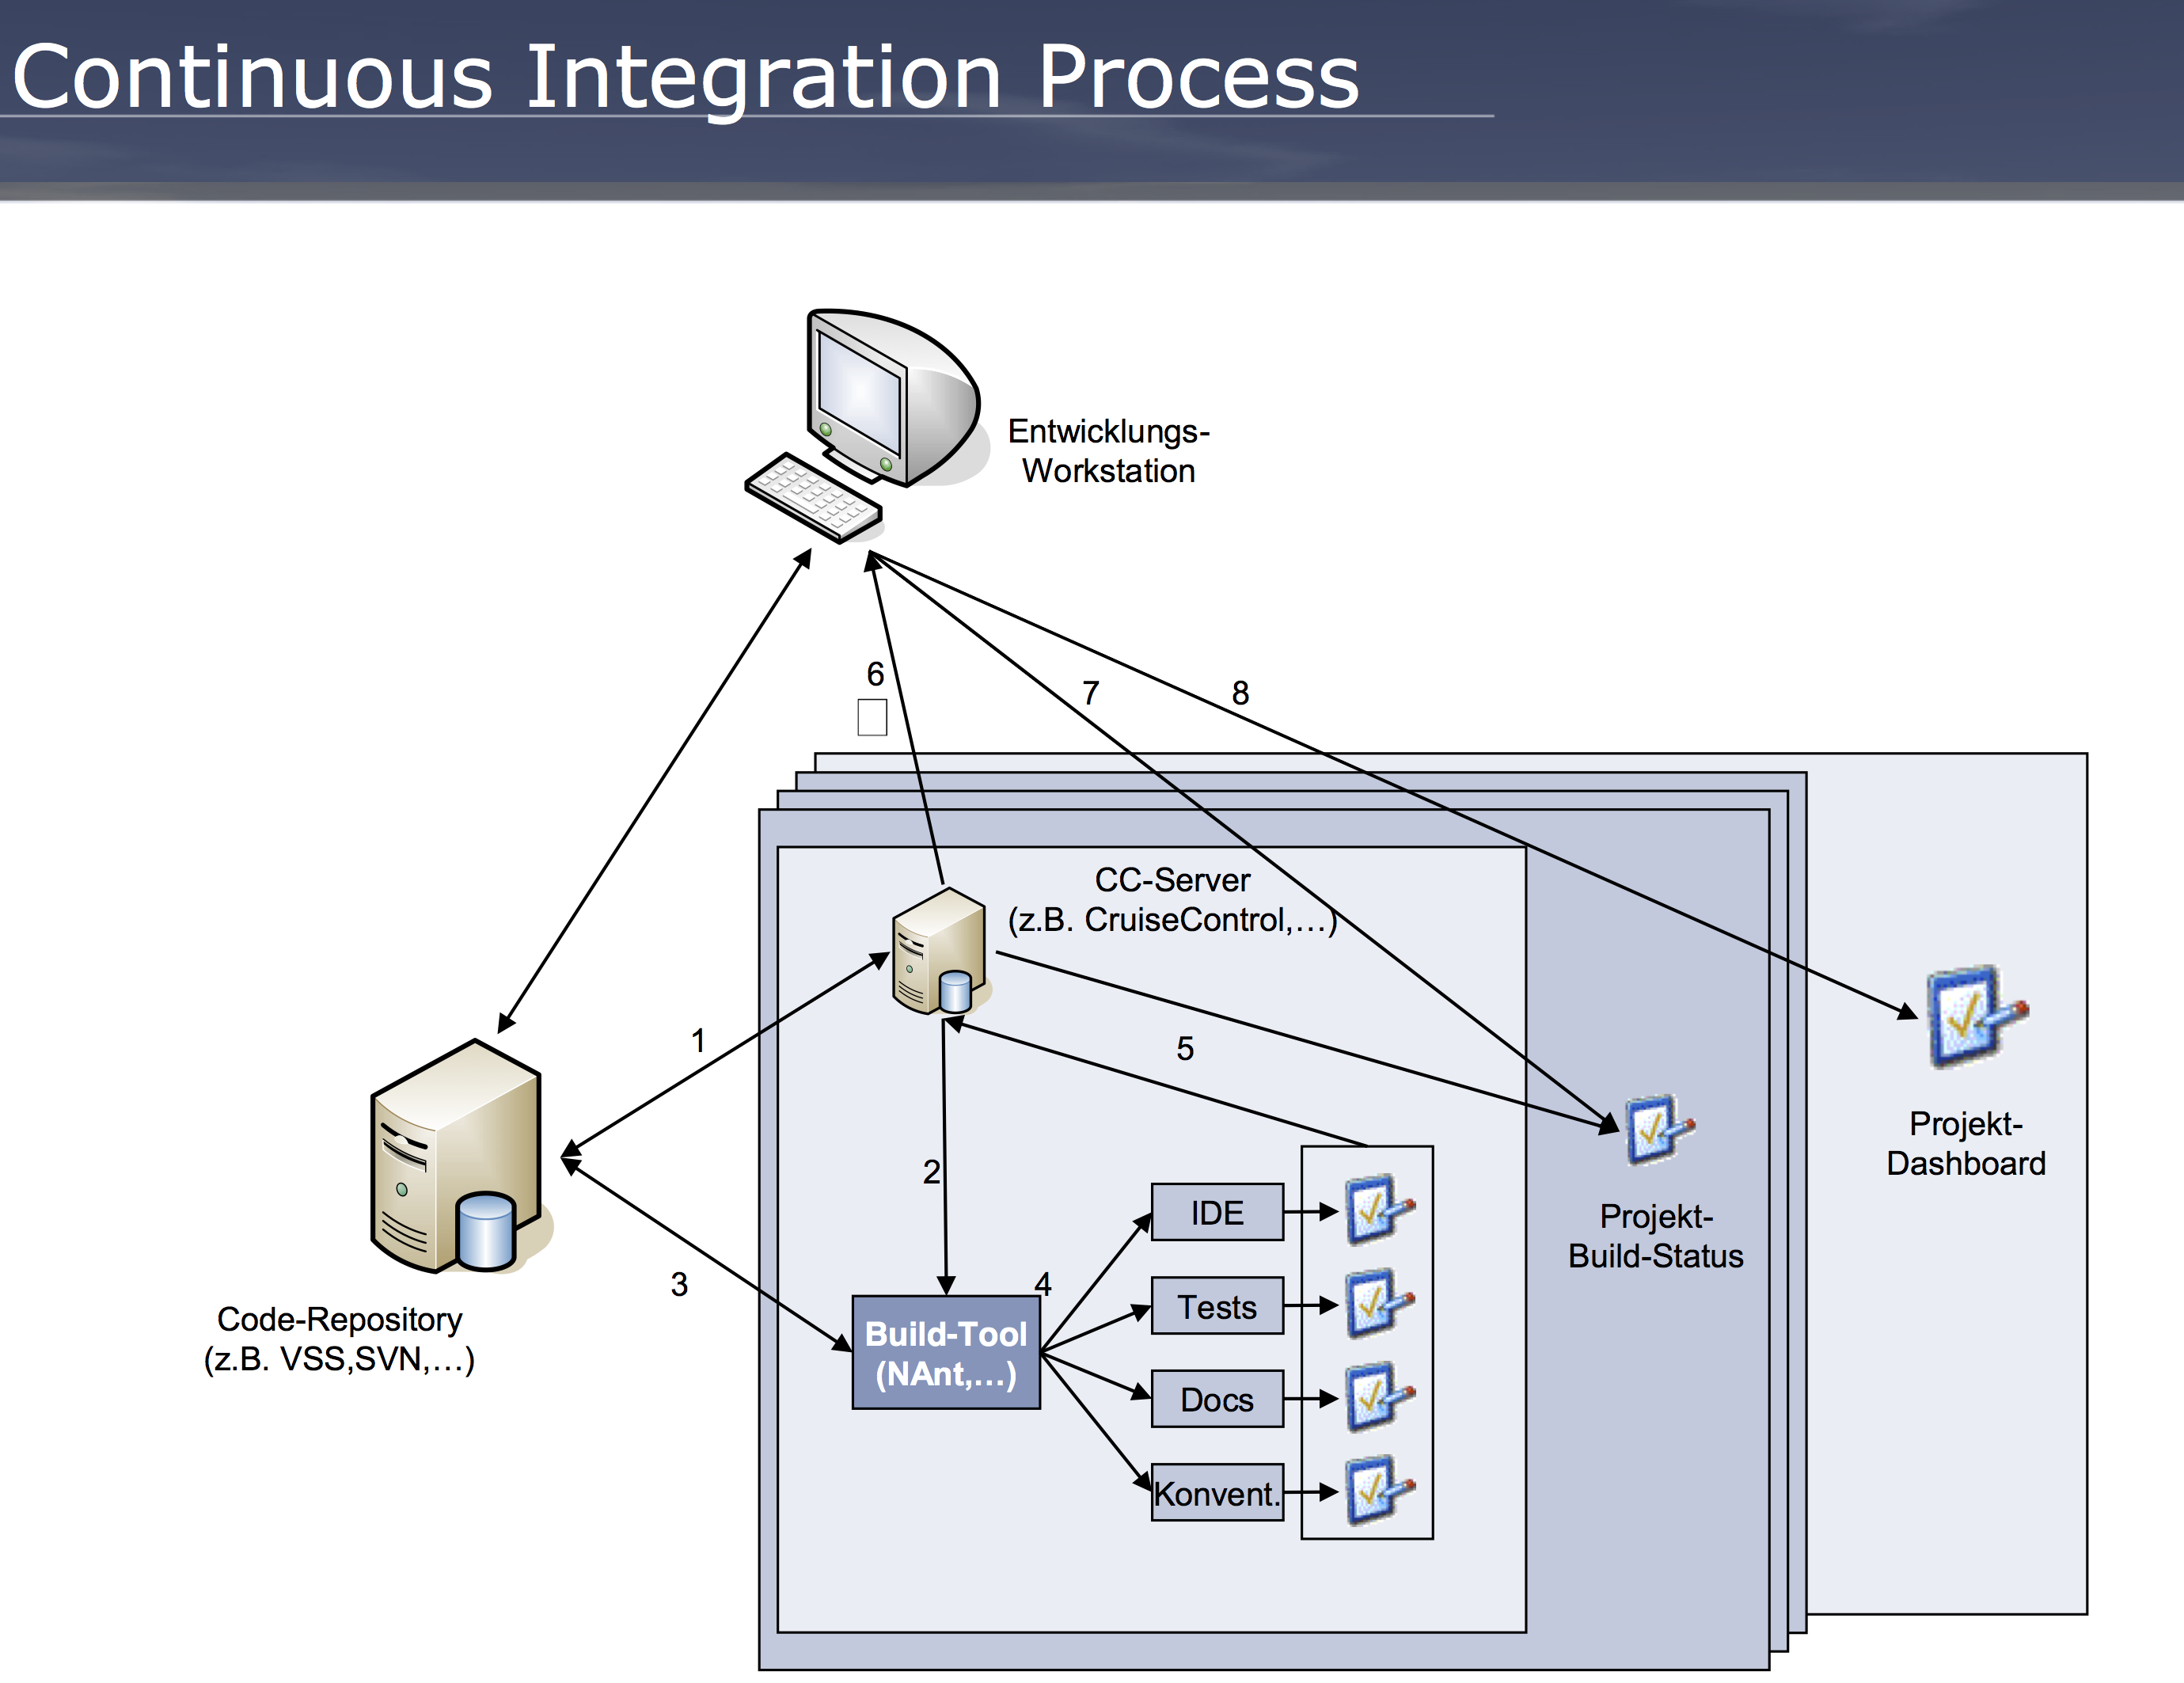
\includegraphics[width=0.8\textwidth]{img/continuousintegration.png}
	\caption{Continuous Build Prozess eines Softwareprojekts nach \cite{build-continuous}}
\label{fig:ci}
\end{figure}

\section{Die Kosten eines fehlgeschlagenen Builds}
Was passiert wenn der Build Prozess fehlschlägt, weil aus welchen Gründen auch immer die Abhängigkeiten nicht korrekt definiert wurden?
\\
Man unterscheidet hierbei bei den Fehlerentstehung zwischen einem \textit{Loud failure}, einem \textit{Silent failure} und einem \textit{Intentional failure}.
Der Loud failure ist ist der Zustand, wenn der Kompiler eine Datei nicht übersetzt, oder das Linking nicht korrekt ist und den Build zum Abbruch bringt.
Der Silent failure ist im Regelfall ein schwer zu findender Fehler, denn der Build war hier erfolgreich, aber der gewünschte Output ist nicht korrekt, weil \acs{z. B.} ein geänderter Code nicht re-kompiliert oder eine alte Bibliothek verwendet wurde.
\\
Der dritte Fehler, der Intentional failure, der vermutlich am  schwersten zu finden ist, entsteht, wenn der Quellcode Backdoors, \acs{etc.} enthält. \cite{software-analysis}

\section{Effektiver Build}
Wie kann man diesen Build Prozess denn nun verbessern, wenn oft etwas schief geht oder der Build Prozess sehr lange dauert?
\\
Folgende simple Antworten sind hierbei zu finden, \cite{software-analysis}:
\begin{itemize}
	\item Verbesserung der Qualität der Software
	\item Reduzierung von verschwendeter Zeit
	\item Verhinderung von Sicherheitsrisiken 
	\item Compliance Vorgaben einhalten 
\end{itemize}
